\documentclass[10pt,twocolumn,letterpaper]{article}

\usepackage{cvpr}
\usepackage{times}
\usepackage{epsfig}
\usepackage{graphicx}
\usepackage{amsmath}
\usepackage{amssymb}

% Include other packages here, before hyperref.

% If you comment hyperref and then uncomment it, you should delete
% egpaper.aux before re-running latex.  (Or just hit 'q' on the first latex
% run, let it finish, and you should be clear).
\usepackage[breaklinks=true,bookmarks=false]{hyperref}

\cvprfinalcopy % *** Uncomment this line for the final submission

\def\cvprPaperID{****} % *** Enter the CVPR Paper ID here
\def\httilde{\mbox{\tt\raisebox{-.5ex}{\symbol{126}}}}

% Pages are numbered in submission mode, and unnumbered in camera-ready
%\ifcvprfinal\pagestyle{empty}\fi
\setcounter{page}{4321}
\begin{document}

%%%%%%%%% TITLE
\title{\LaTeX\ Author Guidelines for CVPR Proceedings}

\author{First Author\\
Institution1\\
Institution1 address\\
{\tt\small firstauthor@i1.org}
% For a paper whose authors are all at the same institution,
% omit the following lines up until the closing ``}''.
% Additional authors and addresses can be added with ``\and'',
% just like the second author.
% To save space, use either the email address or home page, not both
\and
Second Author\\
Institution2\\
First line of institution2 address\\
{\tt\small secondauthor@i2.org}
}

\maketitle
%\thispagestyle{empty}

%%%%%%%%% ABSTRACT
\begin{abstract}
   The ABSTRACT is to be in fully-justified italicized text, at the top
   of the left-hand column, below the author and affiliation
   information. Use the word ``Abstract'' as the title, in 12-point
   Times, boldface type, centered relative to the column, initially
   capitalized. The abstract is to be in 10-point, single-spaced type.
   Leave two blank lines after the Abstract, then begin the main text.
   Look at previous CVPR abstracts to get a feel for style and length.
\end{abstract}

%%%%%%%%% BODY TEXT
\section{Introduction}

Please follow the steps outlined below when submitting your manuscript to
the IEEE Computer Society Press.  This style guide now has several
important modifications (for example, you are no longer warned against the
use of sticky tape to attach your artwork to the paper), so all authors
should read this new version.

%-------------------------------------------------------------------------

\section{Background}

Neural networks can be used for image classification. With the appropriate back propagation (BP) algorithm and the right loss fiction the network eventually will be able to conjure weights that encapsulate some pattern that can differentiate between different classes. neural networks do have a disadvantage since the image have to be flattened to be used in neural network all the spatial features have been lost and the network will have to be bigger to obtain high performance. But with convolutional neural network (CNN) the spatial features can be maintained and work with CNN. and that ability to gives CNN the upper hand comparing it to a neural network \cite{cnn_1_lee}.

 Higher performance in terms of accuracy can be achieved by using a ResNet architecture. the more complex the pattern the more complex the model needs to be for it to approximate the pattern. in deep learning a more complex model equates ( not always but generally true) to a model with more parameters. the number of filters and the size can be increased the meet the demand complexity of the data. unfortunately in bigger CNN models gradients often get smaller and  smaller  as  the  algorithm  progresses down to  the  lower  layers. As  a  result, the Gradient Descent update leaves the lower layer connection weights virtually unchanged, and training never converges to a good solution. in that instances that's called gradient vanishing and when the opposite happens its gradient exploding problem \cite{pmlr-v9-glorot10a}. Such problems can be mitigated using different activation functions with using  clever initialization techniques such as Glorot and He Initialization. Alternatively with the introduction of ResNet architecture allowed for training of large and deep CNN models by using the residual block \cite{ResNet}.


\section{Methodology}

\subsection{CNN}
The main idea behind CNN is using kernels as a combination of estimators. the BP algorithm shall find the right combination of filters or kernels that can abstract and learn high to low level features from the data. to illustrate the idea clearly in figure \ref{fig:blur} the input image have been blurred by applying a blur kernel. the input image can be considered 2D matrix assuming the image has been normalized by multiplying each 3*3 subset of  with a 3*3 kernel as illustrated in figure \ref{fig:blur_math}. 


\begin{figure}[h!]
  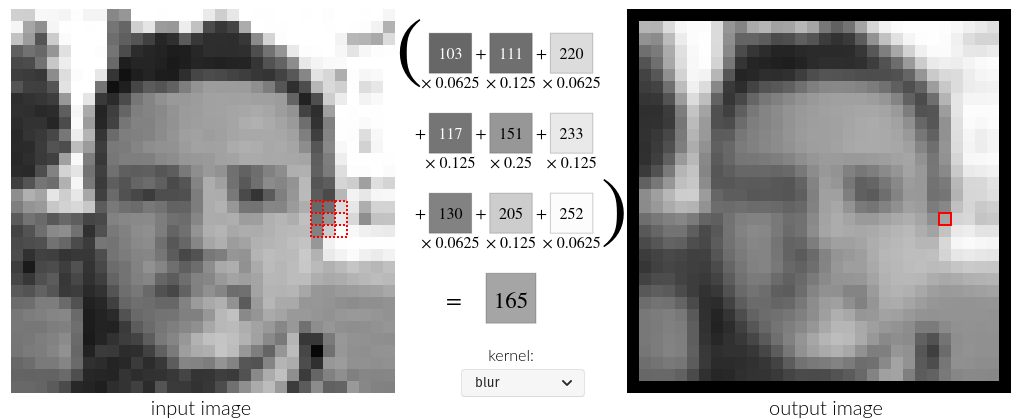
\includegraphics[width=\linewidth]{blur.png}
  \caption{Blur kernel}
  \label{fig:blur}
\end{figure}

\begin{figure}[h!]
  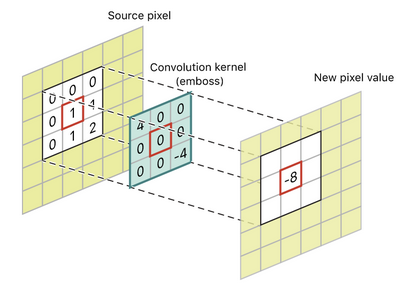
\includegraphics[width=\linewidth]{blur_math.png}
  \caption{applying a kernel}
  \label{fig:blur_math}
\end{figure}

In CNN the values for the kernels are unknown that's what the BP algorithm is trying to obtain. Setting the size of the kernel or the filters and the numbers of the kernels the BP algorithm using Gradient Descent like algorithm will hopefully converge into set of filters that can detect features then using neural network at the of the CNN network for classification.
\begin{figure}[h!]
  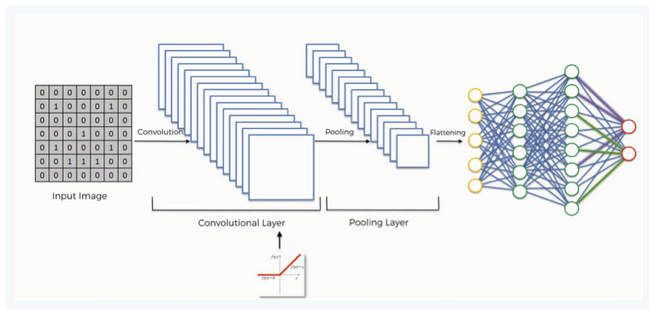
\includegraphics[width=\linewidth]{cnn_nn.png}
  \caption{CNN Network}
  \label{fig:cnn_nn}
\end{figure}


\subsection{VGGNet}

The VGGNet was developed by Simonyan and Zisserman \cite{VGGNet}. The VGG network is famous for its simplicity. it consists of (3*3) convolution blocks stacked on top of each others and as you traverse down the network stack the number of filters increases in figure \ref{fig:VGG_ARC}. 
\begin{figure}[h!]
  \includegraphics[width=\linewidth]{vgg_arc.png}
  \caption{VGG architectures}
  \label{fig:VGG_ARC}
\end {figure}

Training VGG network is extremely difficult and tedious. The original authors had to utilize pre-training to train smaller size of VGG and then use that as a backbone for bigger VGG networks. that was the only way at that time to train VGG network assuming using random initialization for the weights. but Xavier and Yoshua \cite{pmlr-v9-glorot10a} \& Dmytro and Jiri Matas \cite{ini_imp} demonstrated that such training scheme isn't  a must. Using an appropriate initialization technique and swapping to the non-saturating activation function can eliminate the need for pre-training VGG or deep neural network in general. 

\subsubsection{Mini VGG Implementation}
The original VGGNet was designed for ImageNet competition. the image size was 224 * 224 which is different from CIFAR-10 images. my implementation is similar to VGG11 as seen if Figure \ref{fig:VGG_ARC} with smaller number of filters for each VGG block. other layer such as drop out and batch normalization have been utilized to combat over-fitting and stabilize the network.  

%\begin{figure}[h!]
%  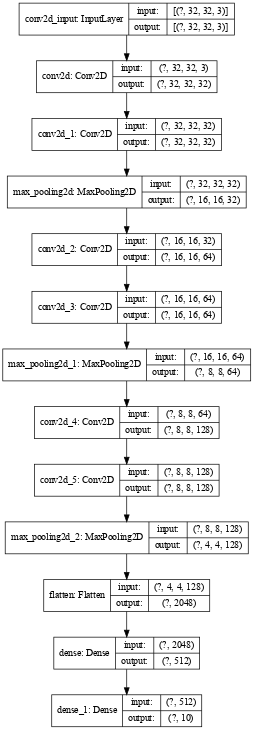
\includegraphics[width=\linewidth, height=10cm]{VGG_3block.png}
%  \caption{Mini VGG Implementation}
%  \label{fig:VGG_IMPLE}
%\end{figure}











{\small
\bibliographystyle{ieee_fullname}
\bibliography{egbib}
}

\end{document}
